  \documentclass{webquiz} 
 	\usepackage[dvipdfmx]{graphicx}
	\DeclareGraphicsExtensions{.png}

     \title{Quiz 1: Estimation models - Scaling laws} 
 
     \UnitCode{MATH1001} 
     \UnitName{Differential Calculus} 
     \UnitURL{/u/UG/JM/MATH1001/} 
     \QuizzesURL{/u/UG/JM/MATH1001/Quizzes/} 
 
     \begin{document} 
 
     \begin{discussion}[Recall on scaling laws][]\\ 
     \newline
       Assumptions : 
     \begin{minipage}[t]{.8\textwidth}
    \begin{itemize} 
     \item  Geometrical similarity  
     \item  Material similarity
     \item  One dominant phenomena
     \end{itemize}
      \end{minipage}
  

	Mathematical form:		$y=kL^a $ \\
				with k function of reference and  a of physical effect

Notation:			$y^*=L^*a$

Obtention ways:	
\begin{minipage}[t]{.8\textwidth}
\begin{itemize} 
     \item  direct manipulation of equations 
     \item  dimensional analysis and Buckingham theorem
     \item  One dominant phenomena
     \end{itemize}
\end{minipage}
Components:           One main design driver express by a constant stress X*=1
        \begin{center} 
        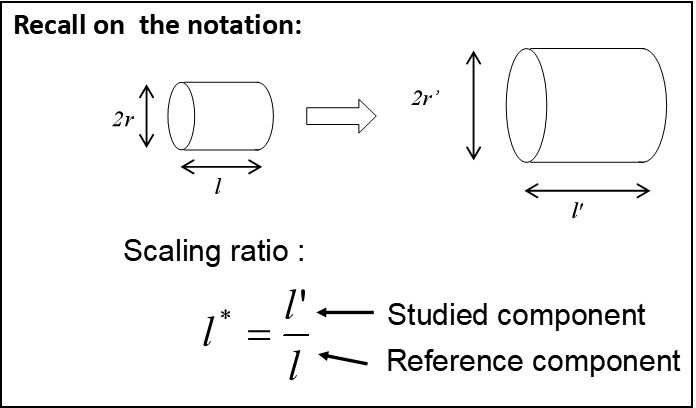
\includegraphics[height=90mm]{Picture1.png}
        \end{center}
     \end{discussion} 
 
  
   \begin{question} 
    We assume to have similarity on all geometrical parameters :  $r^* = d^* = …=  l^*$ \\
    \newline
	Give evolutions of areas : 
     \begin{choice}
      \incorrect  $ l^*$
      \incorrect  $ l^{*^2}$ 
      \incorrect $ l^{*^{-2}}$ 
      \correct  $ l^{*^{\frac{1}{2}}}$ 
     \end{choice} 
   \end{question}
     
   \begin{question} 
    We assume to have similarity on all geometrical parameters :  $r^* = d^* = …=  l^*$ \\
    \newline
	Give evolutions of volumes : 
     \begin{choice}
      \incorrect  $ l^*$
      \incorrect  $ l^{*^2}$ 
      \incorrect  $ l^{*^3}$ 
      \incorrect $ l^{*^{-3}}$ 
      \correct  $ l^{*^{\frac{1}{3}}}$ 
     \end{choice} 
   \end{question}
   
   \begin{question} 
     We assume to have similarity on all geometrical parameters :  $r^* = d^* = …=  l^*$ \\
    \newline
	Give evolutions of masses : 
     \begin{choice}
      \incorrect  $ l^*$
      \incorrect  $ l^{*^2}$ 
      \incorrect  $ l^{*^3}$ 
      \incorrect $ l^{*^{-3}}$ 
      \correct  $ l^{*^{\frac{1}{3}}}$ 
     \end{choice} 
   \end{question}
     \begin{question} 
   We assume to have similarity on all geometrical parameters :  $r^* = d^* = …=  l^*$ \\
    \newline
	Give evolutions of intertias : 
     \begin{choice}
      \incorrect  $ l^{*^2}$ 
      \incorrect  $ l^{*^3}$ 
         \incorrect  $ l^{*^4}$
      \incorrect $ l^{*^{5}}$ 
      \correct  $ l^{*^6}$ 
     \end{choice} 
   \end{question}
     \end{document}
      